\documentclass[a4paper,11pt]{article}

\usepackage{subfigure}
\usepackage{pgfplots}
\usepackage{tikz}
\usepackage[top=3cm,bottom=3cm,left=2.5cm,right=2.5cm]{geometry}

\begin{document}

\begin{figure}
	\centering
	\subfigure[$500$ epochs with batch size $100$.]{
		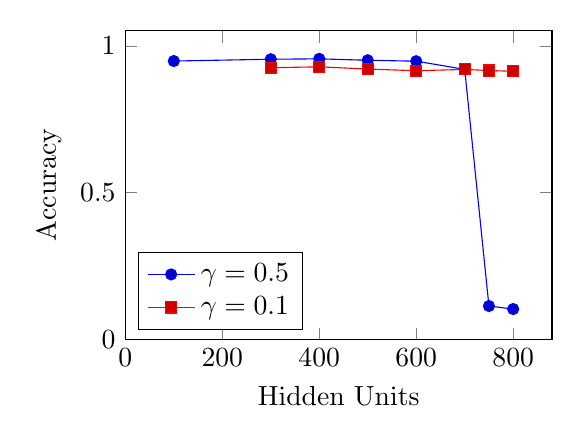
\begin{tikzpicture}
			\begin{axis}[height=5.5cm,width=7cm,ylabel=Accuracy,xlabel=Hidden Units,xmin=0,ymin=0,legend pos=south west]
				\addplot+[blue] coordinates{(100,1-0.0519)(300,1-0.0457)(400,1-0.0444)(500,1-0.0492)(600,1-0.0524)(700,1-0.0801)(750,1-0.8865)(800,1-0.8968)};
				\addlegendentry{$\gamma = 0.5$}
				\addplot+[red] coordinates{(300,1-0.0747)(400,1-0.0716)(500,1-0.0791)(600,1-0.0849)(700,1-0.0804)(750,1-0.0842)(800,1-0.0868)};
				\addlegendentry{$\gamma = 0.1$}
			\end{axis}
		\end{tikzpicture}
		\label{subfig:results-units}
	}
	\subfigure[$500$ epochs with learning rate $\gamma = 0.5$.]{
		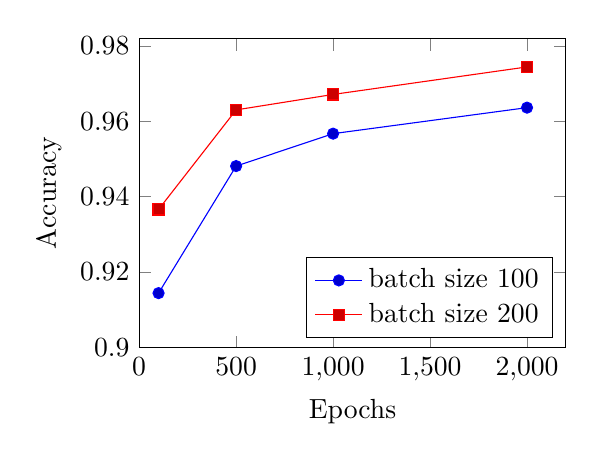
\begin{tikzpicture}
			\begin{axis}[height=5.5cm,width=7cm,ylabel=Accuracy,xlabel=Epochs,xmin=0,ymin=0.9,legend pos=south east]
				\addplot+[blue] coordinates{(100,1-0.0856)(500,1-0.0519)(1000,1-0.0433)(2000,1-0.0364)};
				\addlegendentry{batch size 100}
				\addplot+[red] coordinates{(100,1-0.0634)(500,1-0.0370)(1000,1-0.0329)(2000,1-0.0256)};
				\addlegendentry{batch size 200}
			\end{axis}
		\end{tikzpicture}
		\label{subfig:results-epochs}
	}
\end{figure}

\end{document}